\documentclass[12pt]{article}
\usepackage[english]{babel}
\usepackage{natbib}
\usepackage{url}
\usepackage[utf8x]{inputenc}
\usepackage{amsmath}
\usepackage{graphicx}
\graphicspath{{images/}}
\usepackage{parskip}
\usepackage{fancyhdr}
\usepackage{vmargin}
\usepackage{xcolor}
\usepackage{siunitx}
\usepackage{physics}

\usepackage{caption}
\usepackage{subcaption}

\setmarginsrb{3 cm}{2 cm}{3 cm}{2 cm}{1 cm}{1.5 cm}{1 cm}{1.5 cm}

\title{Lab 09}													% Title
\author{G 03}														% Author
\date{04 june 2019}														% Date

\makeatletter
\let\thetitle\@title
\let\theauthor\@author
\let\thedate\@date
\makeatother

\pagestyle{fancy}
\fancyhf{}
\rhead{\theauthor}
\lhead{\thetitle}
\cfoot{\thepage}
\newcommand{\mis}[3]{(#1 \pm #2) \ #3}
\newcommand{\misp}[3]{(#1 \#3 \pm #2}
\begin{document}

%%%%%%%%%%%%%%%%%%%%%%%%%%%%%%%%%%%%%%%%%%%%%%%%%%%%%%%%%%%%%%%%%%%%%%%%%%%%%%%%%%%%%%%%%

\begin{titlepage}
	\centering
    \vspace*{0.5 cm}
    
\includegraphics[scale = 0.75]{polito.jpg}\\[1.0 cm]				% University Logo
    \textsc{\LARGE Politecnico di Torino}\\[2.0 cm]						% University Name
	\textsc{\Large Digital systems electronics\\ A.A. 2018/2019}\\[0.5 cm]		% Course Code
	\textsc{\Large Prof. G. Masera}\\[0.5 cm]		% Nome del Professore
	\rule{\linewidth}{0.2 mm} \\[0.4 cm]
	{ \huge \bfseries \thetitle \\ \small \thedate}\\
	\rule{\linewidth}{0.2 mm} \\[1.5 cm]
	
	\begin{minipage}{0.4\textwidth}
		\begin{flushleft} \large
			Berchialla Luca\\												%Cognomi e nomi
			Laurasi Gjergji
			\\
			
			Mattei Andrea\\
            Lombardo Domenico Maria\\
            Wylezek Karolina
            
			\end{flushleft}
			\end{minipage}~
			\begin{minipage}{0.4\textwidth}
            
			\begin{flushright} \large
			236032\\													%Matricole
			238259\\
            233755\\
            233959\\
            267219\\
            
		\end{flushright}
        
	\end{minipage}\\[2 cm]
	
\end{titlepage}

%%%%%%%%%%%%%%%%%%%%%%%%%%%%%%%%%%%%%%%%%%%%%%%%%%%%%%%%%%%%%%%%%%%%%%%%%%%%%%%%%%%%%%%%%
\newpage
\section*{Output compare VS Reload}
{
	
	In the following report the Output Compare register and/or auto-reload register can be calculated from the desired asserted flag frequency using the following formula:
	\[F_{X}=\frac{F_{CLK}}{(OC+1)\cdot(ARR+1)}\;\;\;\;\; (1)\] 
	
	Notice that to correctly generate a square wave with a desired frequency $F_{X}$ exploiting the OC or ARR approach, the formula 1 should also be divided by a 2 factor.
}

\section*{1 - Interrupt-based variable frequency square waveform generator}

In the following section a variable frequency square wave has been implemented exploiting the interrupt approach. 
The frequency of the square wave has been set using a potentiometer connected to a GPIO pin of the board. 
The internal ADC converts the analog voltage level provided by the pot into a proper delay:
\[ delta = \frac{OC_{max1} - OC_{min1}}{ADC_{max}} \cdot ADC_{read} + OC_{min1}\]

An interrupt linked to the TIM3 (in OC mode) triggers the toggling of the output pin.
 
\begin{figure}[h!]
	\centering
	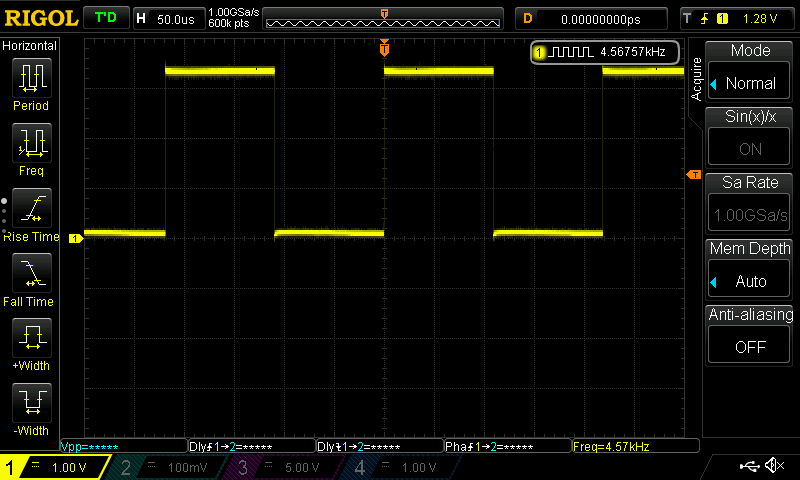
\includegraphics[scale = 0.4]{immagini/DS1Z_QuickPrint10.png}
	\caption{Maximum frequency generated}
\end{figure}
\begin{figure}[h!]
	\centering
	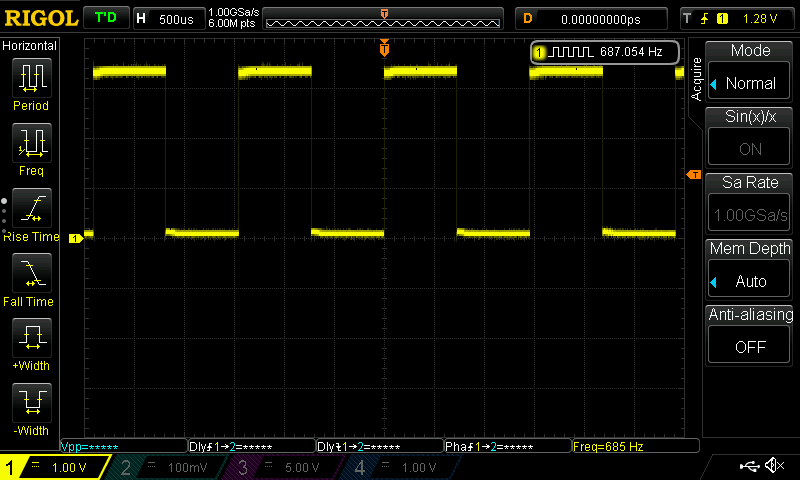
\includegraphics[scale = 0.4]{immagini/DS1Z_QuickPrint11.png}
	\caption{Minimum frequency generated}
\end{figure}

The minimum and maximum frequency of the output waveform generated corresponds to the same values generated in the previous lab, nonetheless they results much more stable and not affected by jitter.

\section*{2.1 - Three interrupts}
In this section a 3-bit clock process has been implemented using the interrupt approach. Three different channels of the same Timer were initially configured in OC mode to produce the given period square wave.
Furthermore the output pin has been configured directly in CubeMX to automatically toggling. 
\begin{figure}[h!]
	\centering
	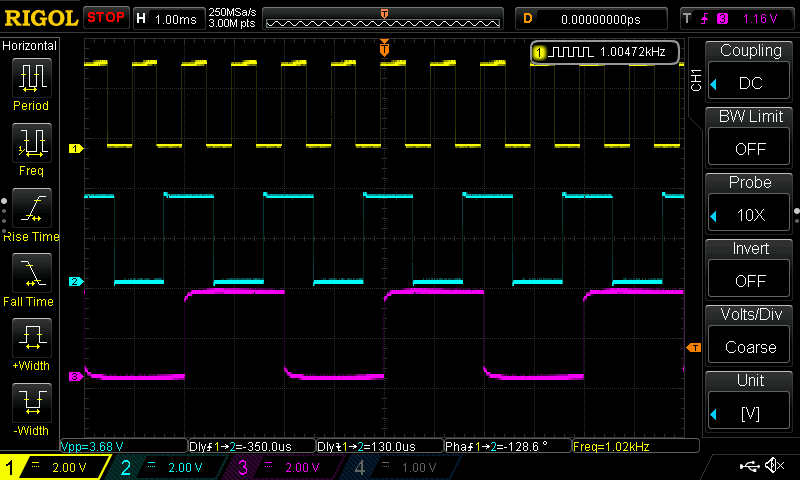
\includegraphics[scale = 0.38]{immagini/DS1Z_QuickPrint13.png}
	\caption{Output square waveforms with different period}
\end{figure}



\section*{2.2 }

The previous project discussed in $section\; 2.1$
has been updated adding the toggling of an LED every time the pushbutton is pressed. 
Another interrupt connected to the GPIO has been implemented and its ISR is responsible for the LED toggling.

The jitter doesn't affect in an appreciable way the correct execution of the program.
\section*{2.3 }

In this section the project 2.1 has been modified. The potentiometer is now responsible for the frequency change of the three square wave, with different ranges.

This time the ADC was used in single conversion mode. Then every new conversion was activated using the channel 2 of TIM2 in OC mode, configured with a period of 500 ms in interrupt mode. 

The figures below show the square waves generated for minimum and maximum achievable frequency, exploiting the potentiometer.


\begin{figure}[h!]
	\centering
	\begin{subfigure}{0.5\textwidth}
		%\centering
		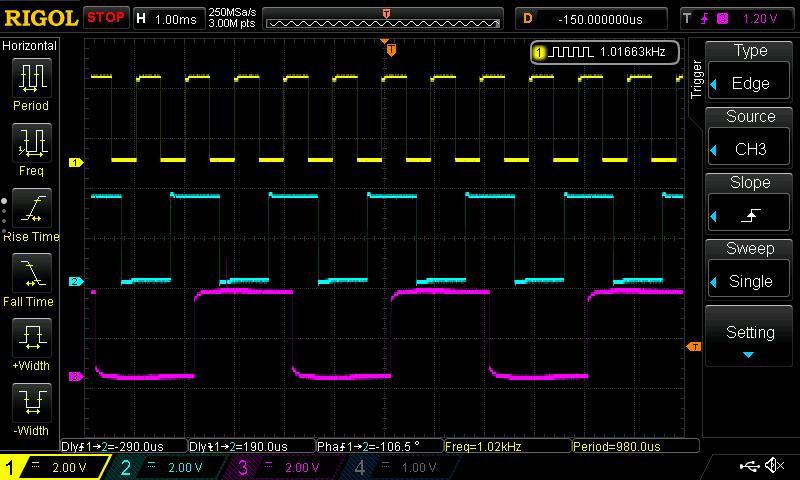
\includegraphics[scale = 0.25]{immagini/DS1Z_QuickPrint14.png}
	\end{subfigure}%
	\begin{subfigure}{0.4\textwidth}
		%\centering
		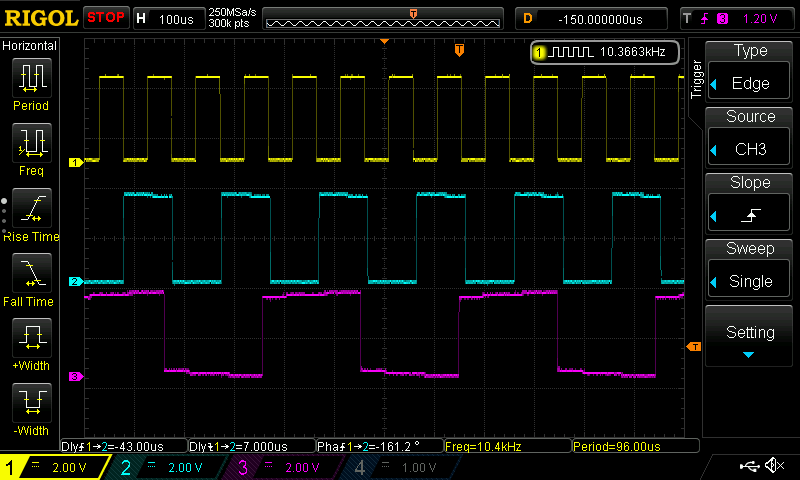
\includegraphics[scale = 0.25]{immagini/DS1Z_QuickPrint15.png}
	\end{subfigure}
	\caption{Minimum and maximum frequency}
\end{figure}



\end{document}




